\chapter{Front End Implementation}

Il FrontEnd fornisce le funzionalità di visualizzazione, inserimento e cancellazione di dati dall'applicazione Sistema Monitoraggio Ambientale. L'applicazione è composta da 5 pagine: Monitoraggio, Parco, Flora, Fauna, Sensori.

\begin{figure}[ht]   
\centering
\includegraphics[scale=0.35]{Img/Menuù.png}
    \caption{Menù dell'applicazione}
    \label{Menu}
\end{figure}

Per utilizzare l'applicazione è presente un menù che guida la navigazione tra le pagine del progetto. Nelle prime tre voci, al momento della selezione si apre un menù a tendina che permette di selezionare il parco, l'animale o la vegetazione desiderata.

\begin{figure}[ht]   
\centering
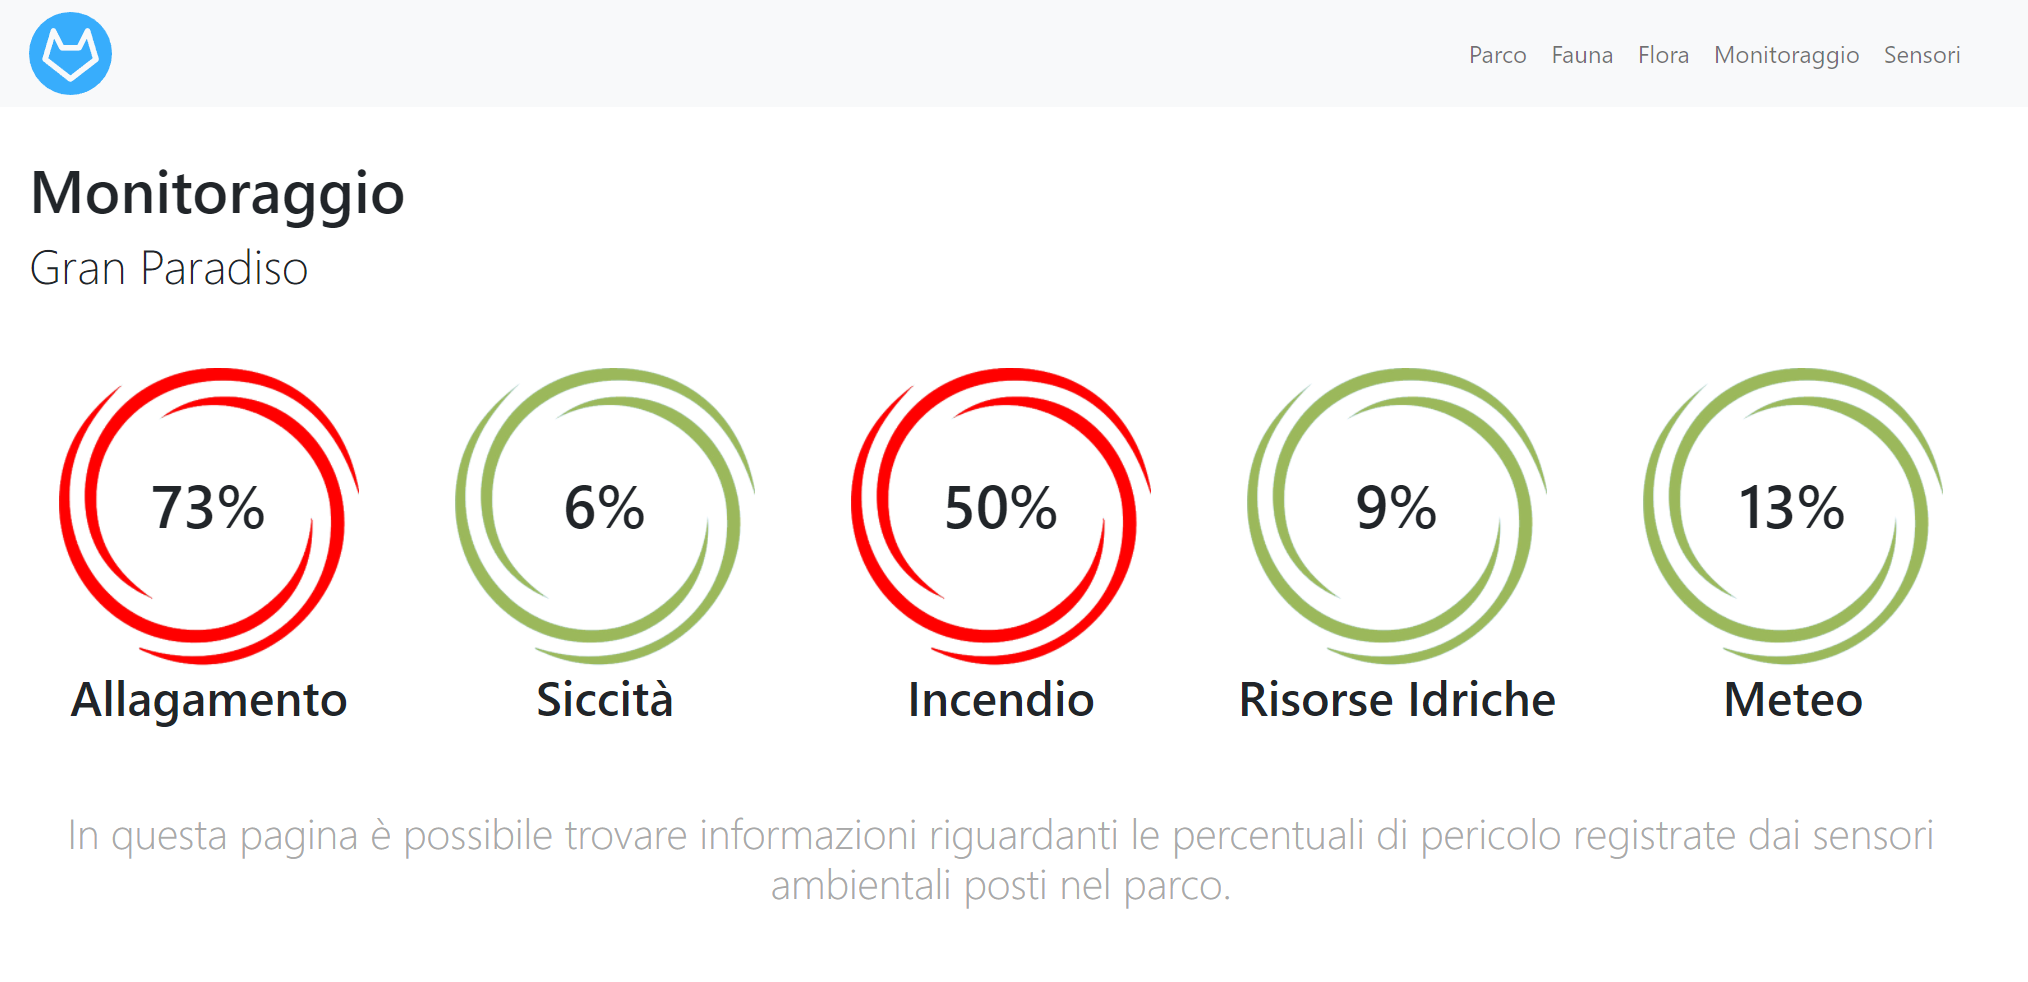
\includegraphics[scale=0.45]{Img/Monitoraggio.png}
    \caption{Pagina di Monitoraggio}
    \label{Monitoraggio}
\end{figure}


Nella Figura \ref{Monitoraggio} si possono visualizzare i livelli di pericolo delle categorie di monitoraggio del parco selezionato. In base al livello raggiunto il colore cambia tra verde, giallo e rosso.

\newpage
\begin{figure}[ht]   
\centering
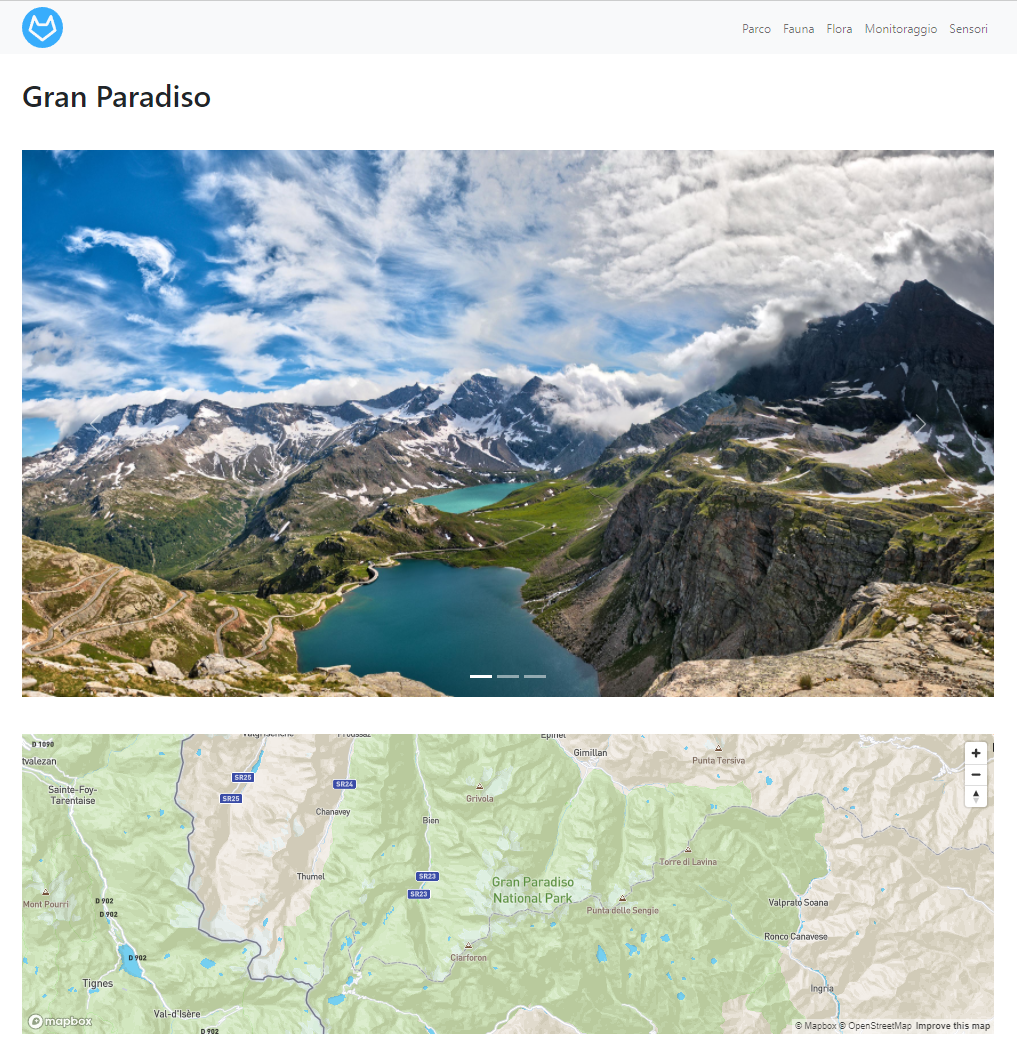
\includegraphics[scale=0.9]{Img/Parco.png}
    \caption{Esempio di Parco selezionato}
    \label{parcoselezionato}
\end{figure}

Nella Figura \ref{parcoselezionato} è possibile visualizzare delle immagini del parco ed una cartina geografica navigabile del suddetto.

\newpage

\begin{figure}[ht]   
\centering
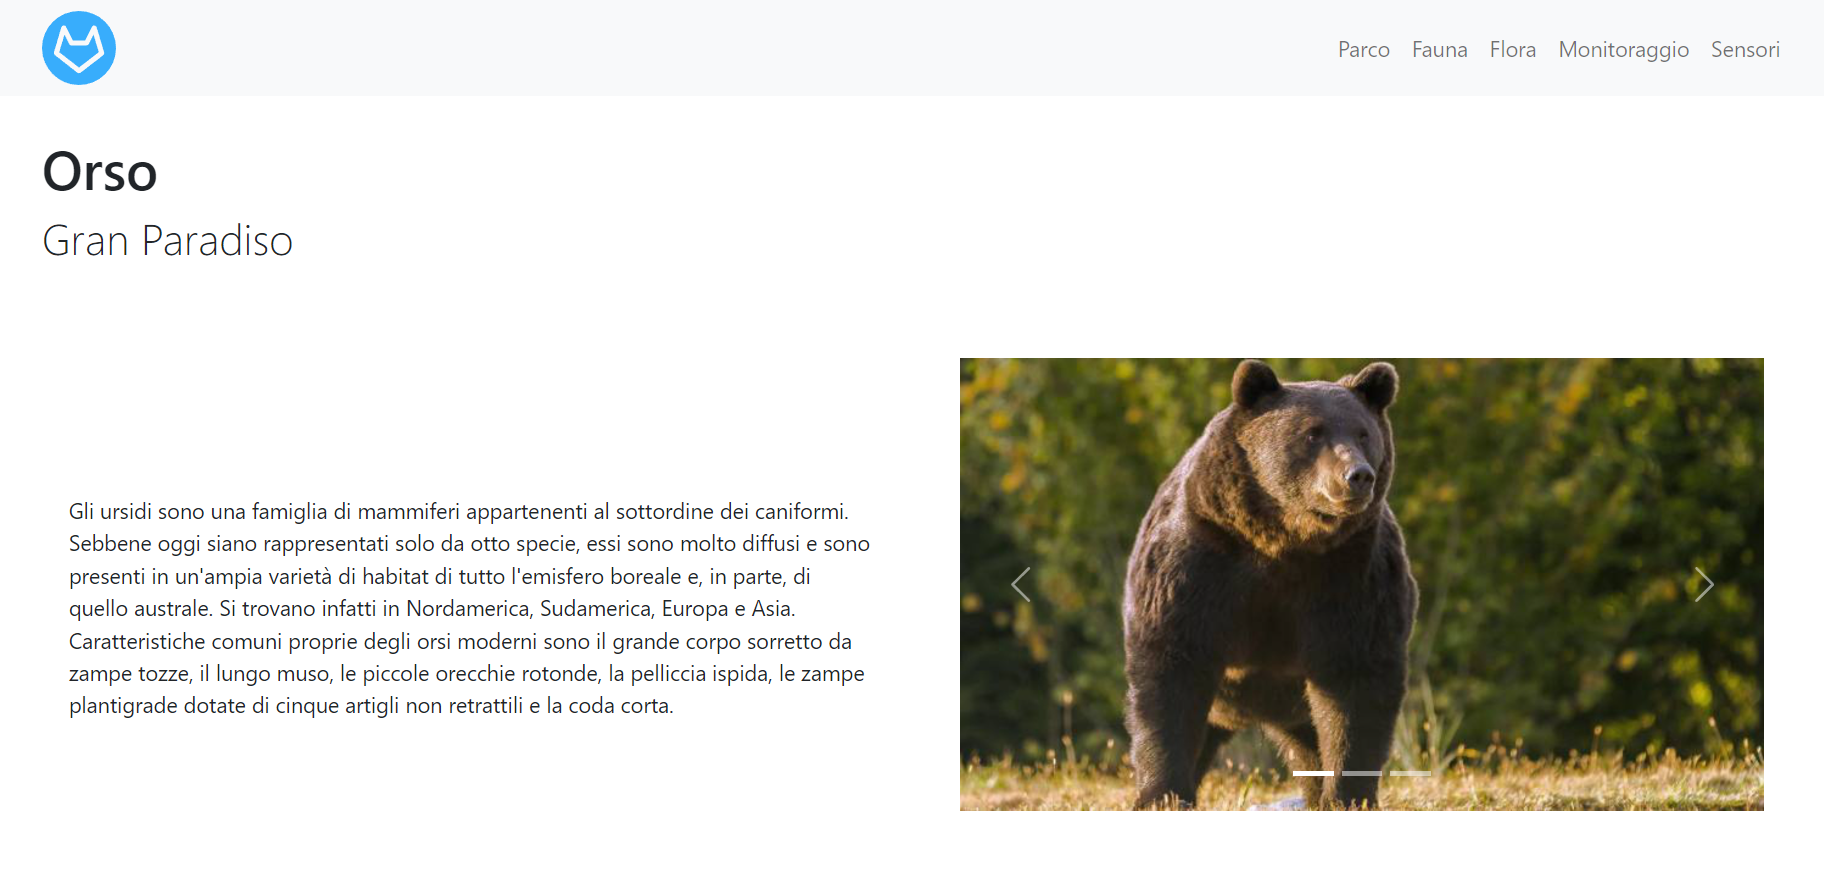
\includegraphics[scale=0.45]{Img/Fauna1.png}
    \caption{Descrizione dell'animale selezionato}
    \label{fauna1}
\end{figure}

\begin{figure}[ht]   
\centering
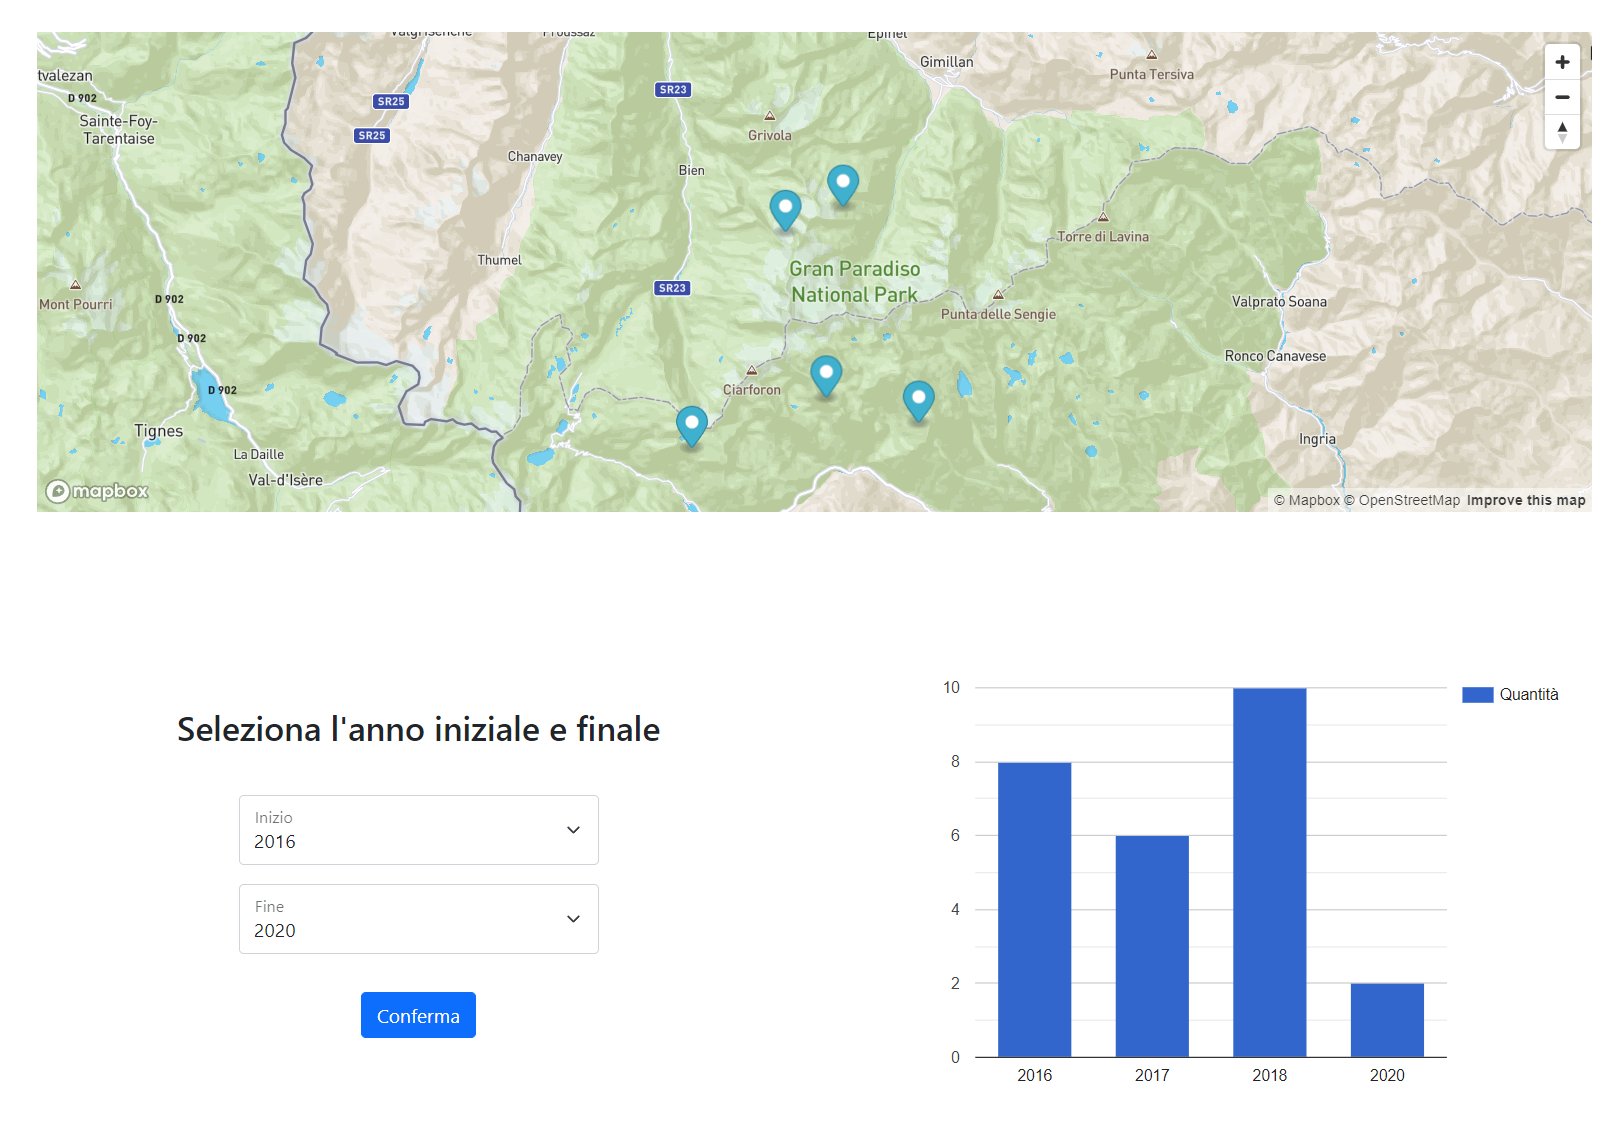
\includegraphics[scale=0.45]{Img/Fauna2.png}
    \caption{Posizione geografica e istogramma della popolazione}
    \label{fauna2}
\end{figure}

Nella figura \ref{fauna1} e \ref{fauna2} si possono visualizzare la descrizione e le immagini dell'animale selezionato. Inoltre è presente una mappa contenente dei marker che tracciano la posizione degli esemplari scelti. Infine si trova un form per inserire l'intervallo di tempo nel quale visualizzare i dati dello storico della popolazione del suddetto.

\begin{multicols}{2}
    \begin{Figure}
        \centering
        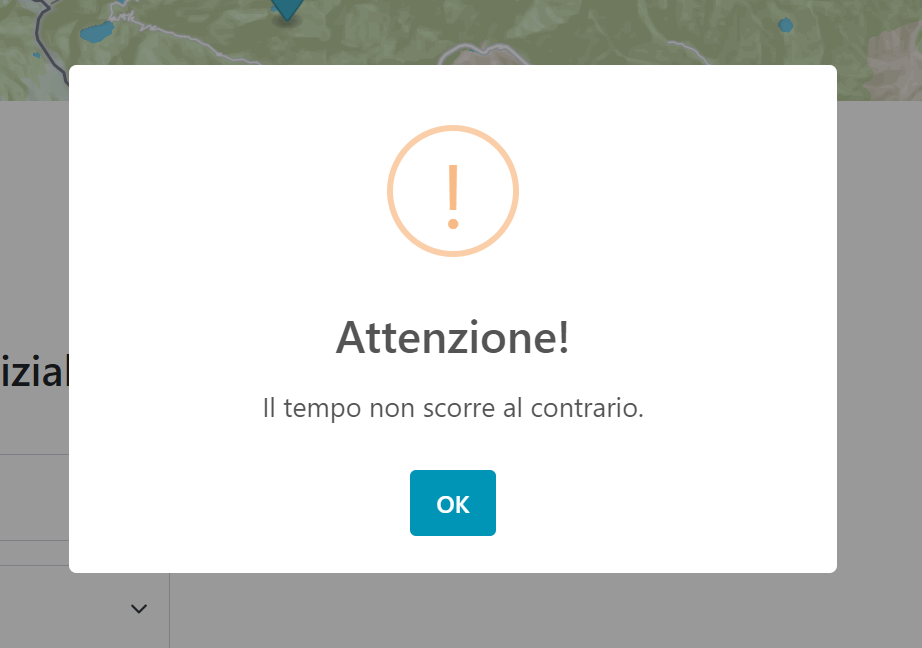
\includegraphics[scale=0.35]{Img/erroreIstogramma.png}
        \captionof{figure}{Pop-up selezione anni errati}
        \label{fig:erroreIstogramma}
    \end{Figure}
    \columnbreak
    Nel caso in cui l'utente selezioni una data di inizio maggiore a quella di fine viene mostrato un pop-up di avvertimento \ref{fig:erroreIstogramma}.
\end{multicols}

\newpage
\begin{figure}[ht]   
\centering
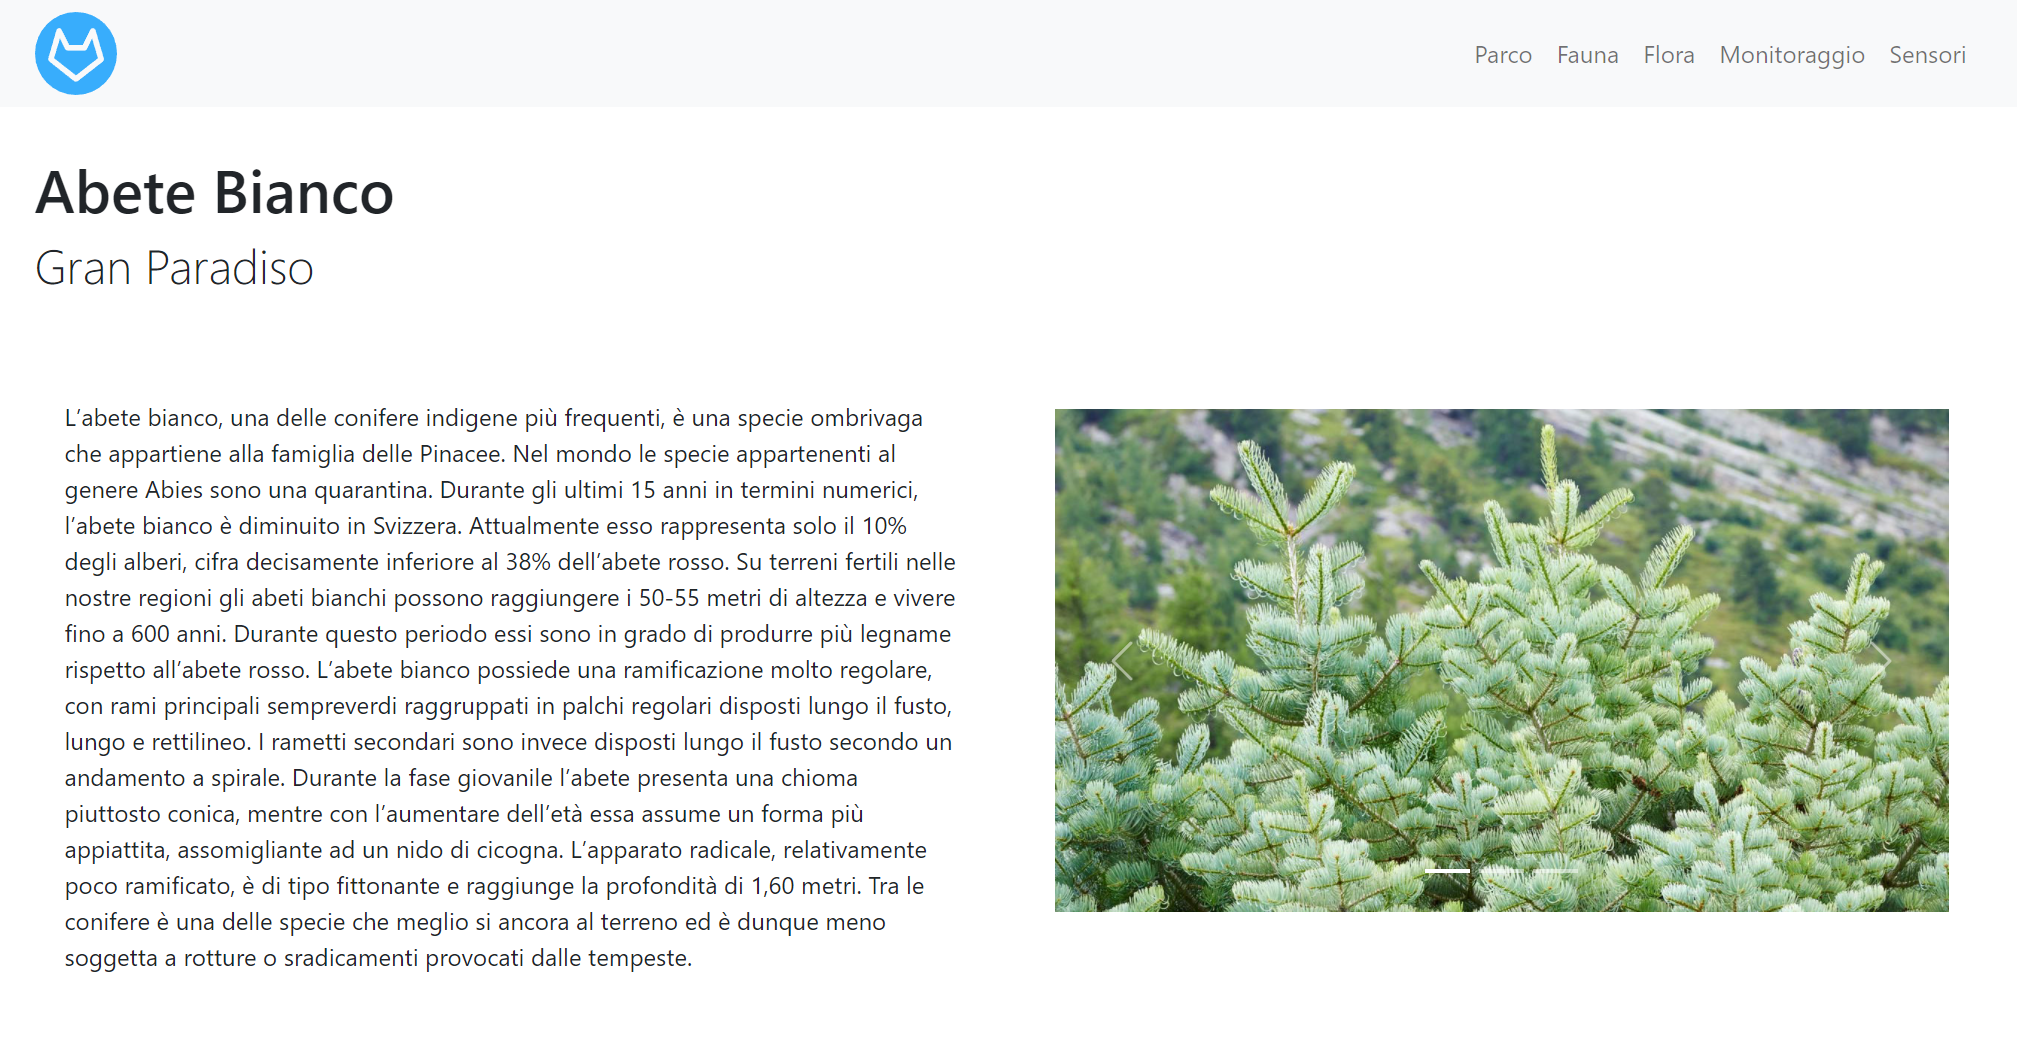
\includegraphics[scale=0.45]{Img/Flora.png}
    \caption{Pagina Flora dell'applicazione Sistema Monitoraggio Ambientale}
    \label{flora}
\end{figure}

Nella figura \ref{flora} si possono visualizzare descrizione ed immagini della specie vegetale selezionata.

\begin{figure}[ht]   
\centering
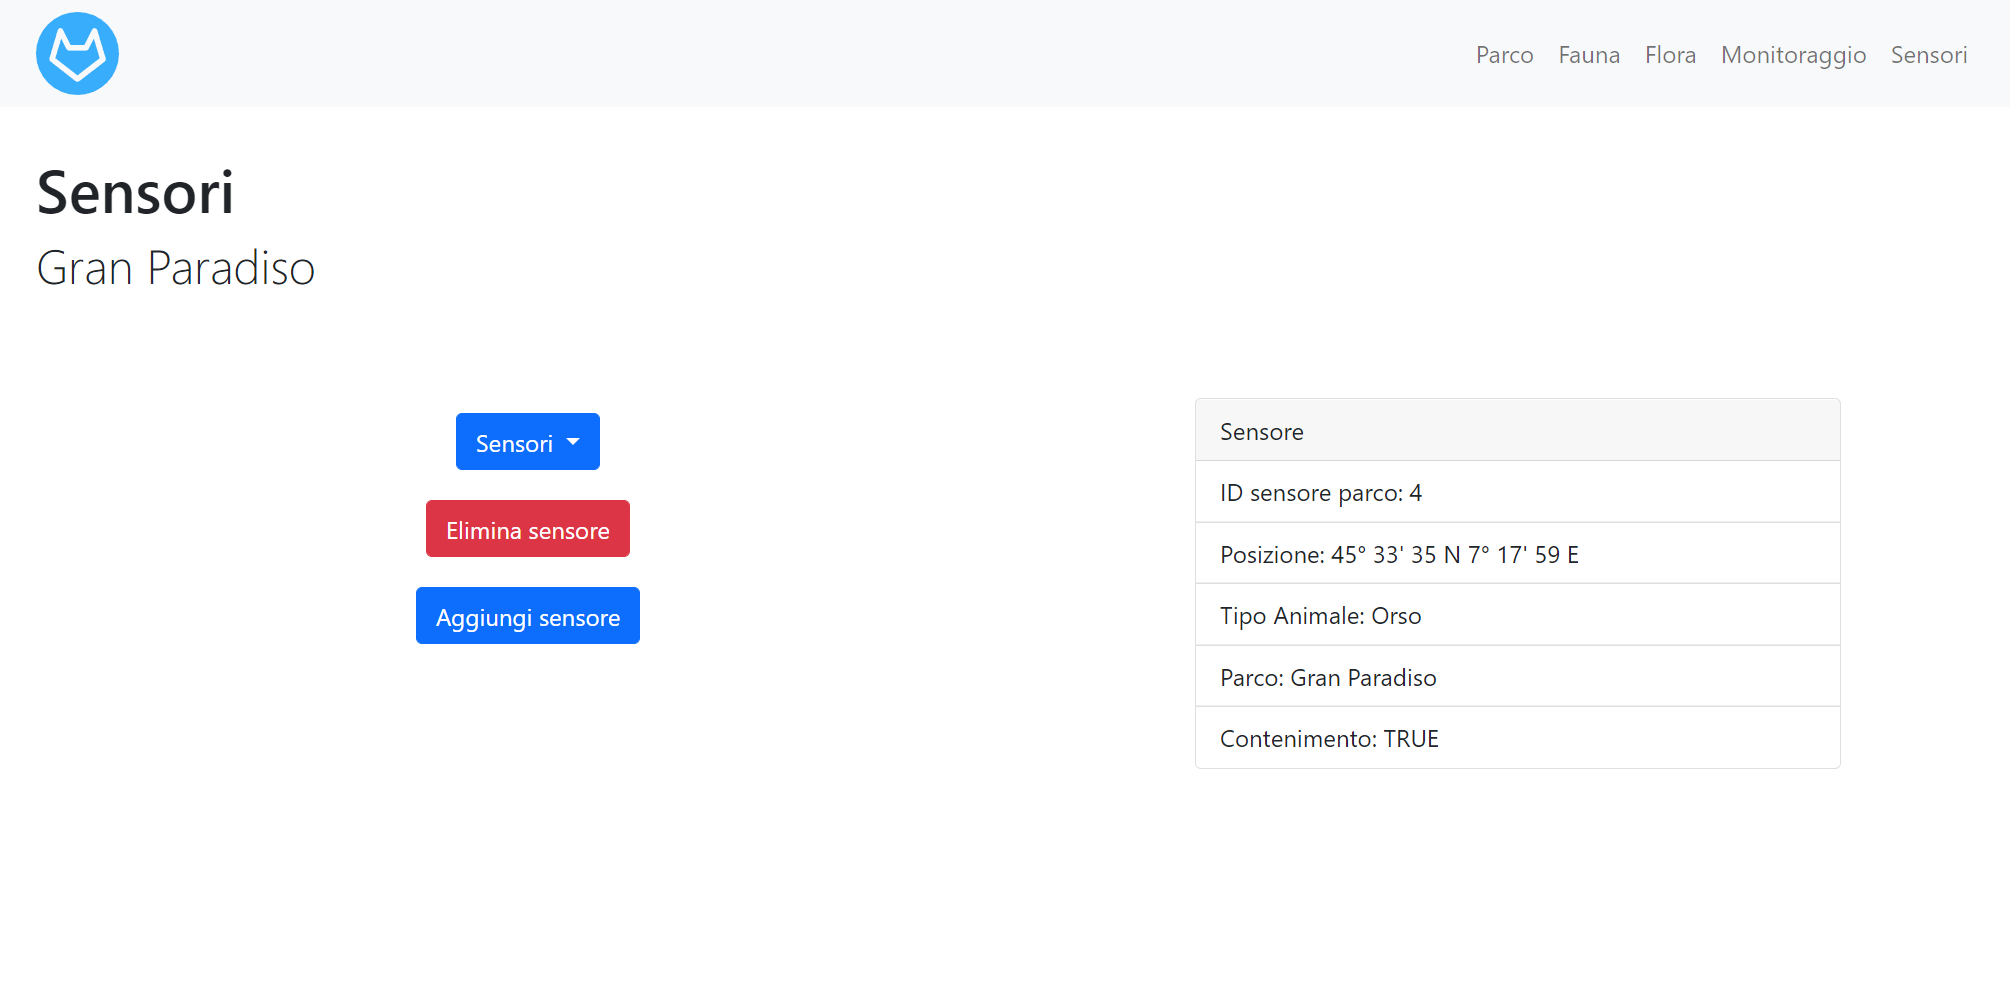
\includegraphics[scale=0.45]{Img/Sensori.png}
    \caption{Pagina dei Sensori}
    \label{sensorilista}
\end{figure}

Nella figura \ref{sensorilista} troviamo nella parte sinistra la possibilità di selezionare, eliminare
ed aggiungere un sensore, mentre nella parte destra una tabella sulla qualche visualizzare i dati del sensore selezionato.
\noindent
L'opzione "Elimina sensore" viene resa disponibile dopo aver selezionato un sensore e permette di eliminare quel preciso sensore dalla lista, notificando l'utente mediante un pop-up.

\newpage
\begin{multicols}{2}
    \begin{Figure}
        \centering
        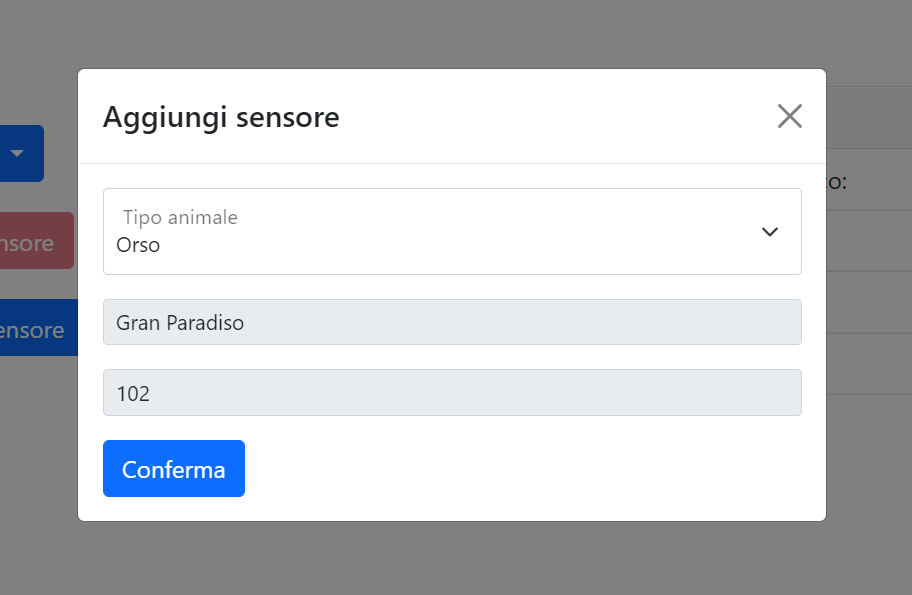
\includegraphics[scale=0.5]{Img/aggiungiSensore.png}
        \captionof{figure}{Form aggiungi sensore}
        \label{fig:formAggiungiSensore}
    \end{Figure}
    \begin{Figure}
        \centering
        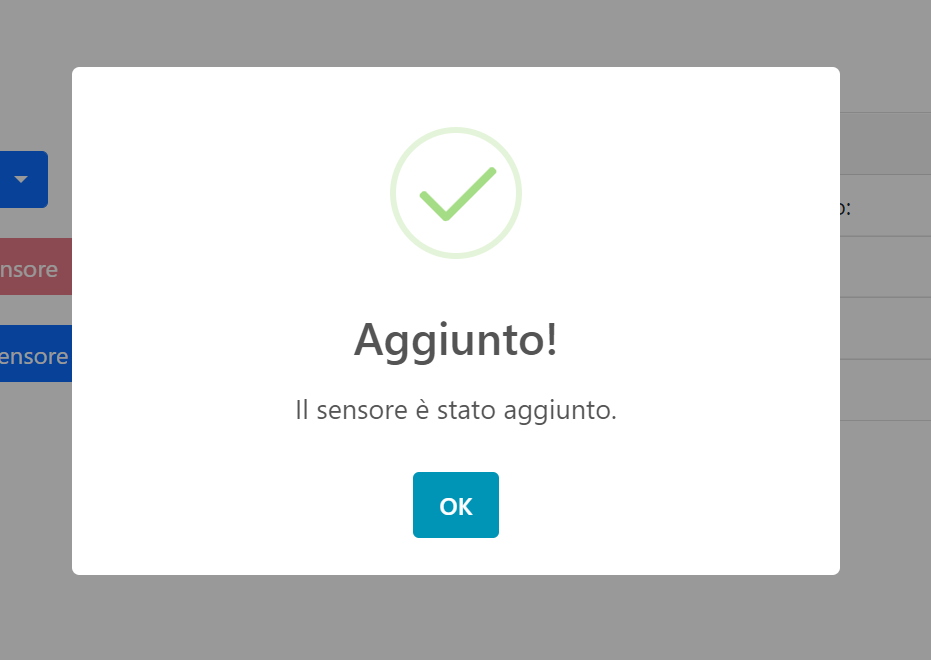
\includegraphics[scale=0.45]{Img/avvenutaAggiunta.png}
        \captionof{figure}{Pop-up conferma}
        \label{fig:avvenutaAggiunta}
    \end{Figure}
\end{multicols}

Nel caso in cui si volesse aggiungere un sensore (figura \ref{fig:formAggiungiSensore}), l'amministratore deve inserire il tipo di animale, mentre 
i campi "Parco" e "ID sensore parco" sono precompilati dal programma, il quale assegna tali valori in base al parco e al numero di sensori presenti in esso nel momento dell'inserimento.

Come definito dallo User Flow al capitolo \ref{capitolo3}, il sistema prevede l'invio di conferma aggiunta sensore (figura \ref{fig:avvenutaAggiunta}) come anche un pop-up che richieda se l'utente è sicuro di voler eliminare un sensore (figura \ref{fig:richiestaEliminazine}) e di seguito l'avvenuta eliminazione (figura \ref{fig:avvenutaEliminazione}).

\begin{multicols}{2}
     \begin{Figure}
        \centering
        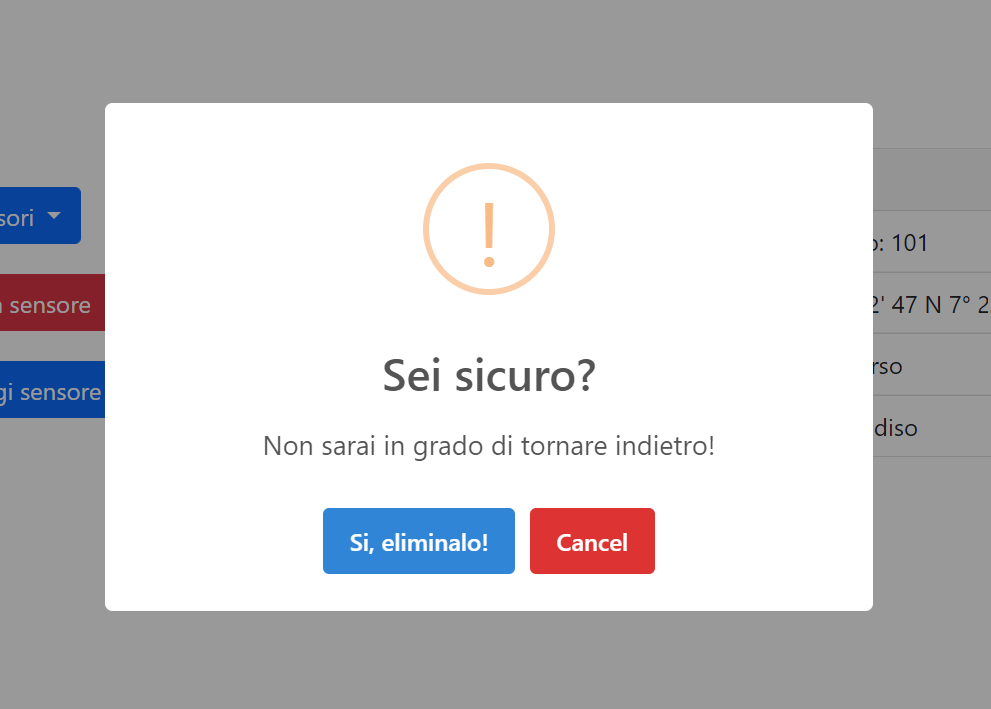
\includegraphics[scale=0.45]{Img/confermaEliminazione.png}
        \captionof{figure}{Form aggiungi sensore}
        \label{fig:richiestaEliminazine}
    \end{Figure}
    \begin{Figure}
        \centering
        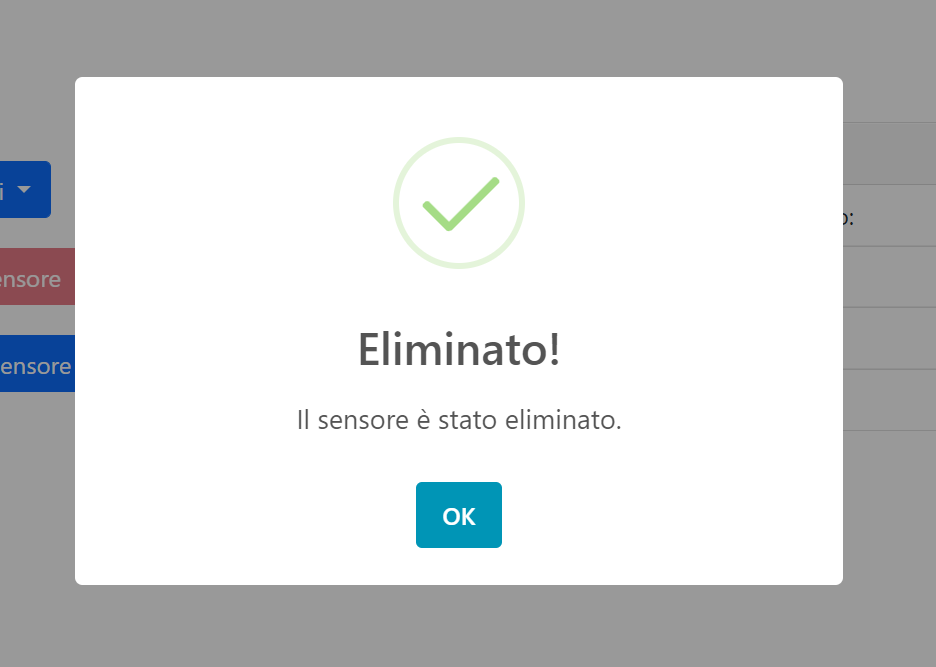
\includegraphics[scale=0.47]{Img/eliminato.png}
        \captionof{figure}{Pop-up conferma}
        \label{fig:avvenutaEliminazione}
    \end{Figure}
\end{multicols}

